\chapter{Задача о сдавливании тонкого нелинейно-вязкопластического слоя}\label{ch:ch4}
Важная группа обобщений классической задачи Прандтля \autocite{Prandtl:1948} связана с усложнением свойств деформируемой среды. Классическая теория пластичности не оперирует физическим временем, его роль играет некоторый неубывающий параметр. Однако реальные процессы неупругого деформирования происходят по нескольким механизмам, и для описания некоторых из них физическое время является необходимым. Одним из них является процесс вязкопластического деформирования, в котором отклик материала зависит от скорости нагружения. В работе \autocites{Georgievsky:2012} обобщено решение классической задачи Прандтля на случай течения вязкопластического материала, характеризующегося пределом текучести и функцией упрочнения. В данной постановке задачи исследуется влияние динамических эффектов в процессе прессования тонкого слоя между сближающимися плитами. Материалы главы содержатся в публикации \fixme{добавить ссылку когда будет статья}.

\section{Постановка задачи и асимптотические разложения}\label{sec:ch4/sec1}

Пренебрегая начальными упругими деформациями, материал, имеющий плотность $\varrho$, полагается несжимаемым вязкопластическим, удовлетворяющим тензорно линейным определяющим соотношениям и скалярному определяющему соотношению  $\sigma_{u} = \sigma_{s} + F(v_{u})$, где $\sigma_{u} = \sqrt{\utilde{s} : \utilde{s}}$ -- интенсивность напряжения, $\utilde{s}$ -- девиатор напряжения, $\sigma_{s}$ -- предел текучести, $v_{u}$ -- интенсивность скоростей деформации, а функция $F$ характеризует нелинейно-вязкопластические свойства материала, причем
\begin{equation}
  \lim_{v_{u}\rightarrow 0}F(v_{u}) = 0.
\end{equation}
В случае линейного упрочнения $F(v_{u}) = 2 m v_{u}$ получаем двухконстантный материал Бингама с динамической вязкостью $m$.

Пусть течение происходит в области
\begin{equation}
  \Omega_{t} = \{-l(t) \le x_{1} \le l(t), -h(t) \le x_{2} < h(t)\},
\end{equation}
с границей $\partial\Omega = \Gamma = \Gamma_{1} \cup \Gamma_{2} \cup \Gamma_{3} \cup \Gamma_{4}$, причем $h(t) \ll l(t)$ для любого $t \ge 0$.
В начальный момент времени область, занятая материалом, имела вид
\begin{equation}
  \Omega_{0} = \{-l_{0} \le x_{1} \le l_{0}, -h_{0} \le x_{2} \le h_{0}\}, \quad \partial\Omega_{0} = \Gamma_{0}
\end{equation}
поэтому в силу несжимаемости $h l=h_{0} l_{0}$.

\begin{figure}[ht]
  \centerfloat{
    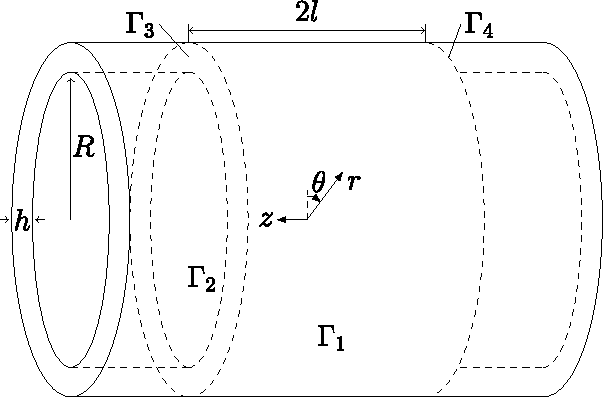
\includegraphics[width=0.6\linewidth]{./ch4/layer}
  }
  \caption{Представление плоского слоя}
  \label{fig:ch4/layer/circle}
\end{figure}
Взаимную скорость сближения плит обозначим $2V$, поэтому кинематическое условие непротекания сквозь границы $\Gamma_{1}$ и $\Gamma_{2}$ имеет вид
\begin{equation}
  \label{eq:ch4/sec1/boundary/kinematic}
  v_{2}\lvert_{x_2\pm h} = \mp V
\end{equation}
Касательная составляющая скорости (в данном случае $v_{1}$) на указанных границах идеальной среды, как известно, не задаётся.

В некоторый момент времени $0 < t < h_{0}/V = t_*$, где $t_*$ -- момент схлопывания слоя, относительно шести функций -- независимых компонент девиатора напряжений $s_{11}$ и $s_{12}$, давления $p$ и компонент скорости $v_{1}$ и $v_{2}$ -- должна выполнятся замкнутая система уравнений динамической теории вязкопластичности:
\begin{subequations}
  \label{eqs:ch4/sec1/general}
  \begin{gather}
    \label{eqs:ch4/sec1/general/motion:1}
    -p_{,1}+s_{11,1}+s_{12,2} = \varrho \left(v_{1;t}+v_{1} v_{1,1} + v_{2} v_{1,2} \right)
    \\
    \label{eqs:ch4/sec1/general/motion:2}
    -p_{,2}-s_{11,2}+s_{12,1} = \varrho \left(v_{2;t}+v_{1} v_{2,1} + v_{2} v_{2,2} \right)
    \\
    \label{eqs:ch4/sec1/general/plasticity}
    \sqrt{s^2_{11}+s^2_{12}}=\sigma_{s} + F(v_{u}), \quad v_{u} = \sqrt{2 v^2_{1,1}+\left(v_{1,2}+v_{2,1}\right)^2 / 2}
    \\
    \label{eqs:ch4/sec1/general/coax}
    s_{11} \left(v_{1,2}+v_{2,1}\right) = 2 s_{12} v_{1,1}
    \\
    \label{eqs:ch4/sec1/general/uncompress}
    v_{1,1}+v_{2,2} = 0
  \end{gather}
\end{subequations}
Кроме выполнения условия \cref{eq:ch4/sec1/boundary/kinematic} на жестких контактирующих поверхностях потребуем, что бы модуль касательного напряжения $s_{rz}$ достигал на границах $\Gamma_{1}$ и $\Gamma_{2}$ своего максимального значения:
\begin{equation}
  \label{eq:ch4/sec1/boundary/force}
  \lvert s_{12}\lvert_{x_2=\pm h} = \mu(x_1) \tau_{s}, \quad 0 < \mu \le 1,
\end{equation}
где $\mu$ -- шероховатость пресса. Абсолютной шероховатости, или полному сцеплению пресса с материалом, соответствует значение $\mu = 1$.

В реальном процессе сжатия слоя границы $\Gamma_{3}$ и $\Gamma_{4}$, естественно, свободны от напряжений, однако в математической постановке рассматриваемой здесь краевой задачи в её классическом варианте данное условие не ставится. Поэтому других, помимо \cref{eq:ch1/sec1/boundary/kinematic, eq:ch1/sec1/boundary/force}, граничных условий в задаче не предполагается, а область вблизи границ $\Gamma_{3}$ и $\Gamma_{4}$ (на расстояниях порядка $h$) трактуется как зона краевого эффекта.

Введем малый параметр $\alpha = \frac{h(t)}{R(t)} \ll 1$ и проведем разложение всех неизвестных величин, входящих в систему уравнений \cref{eqs:ch4/sec1/general}, в ряды по целым степеням параметра:
\begin{subequations}
  \label{eqs:ch4/series}
  \begin{gather}
    v_{1}\left(x_1, x_2, t\right) = V \sum_{k=-N}^{\infty}{\alpha^{k} \; \uindex{v}{k}_{1}}, \quad N \ge 1
    \\
    v_{2}\left(x_1, x_2, t\right) = V \sum_{k=0}^{\infty}{\alpha^{k} \; \uindex{v}{k}_{2}}
    \\
    s_{ij}\left(x_1, x_2, t\right) = \tau_{s} \sum_{k=0}^{\infty}{\alpha^{k} \; \uindex{s}{k}_{ij}}, \quad (ij)\in\{11, 12\}
    \\
    p\left(x_1, x_2, t\right) = \tau_{s} \sum_{k=-M}^{\infty}{\alpha^{k} \; \uindex{p}{k}}, \quad M \ge 1
  \end{gather}
\end{subequations}
Коэффициенты рядов \cref{eqs:ch4/series} -- безразмерны и являются функциями безразмерных координат $\xi_1, \xi_2, \tau$ :
\begin{equation}
  \label{eq:ch4/coordinates}
  \xi_1 = x_1 / l = \alpha x_1 / h, \quad \xi_2 = x_2 / h, \quad \tau = V \frac{t}{h}
\end{equation}
Наличие в \cref{eqs:ch4/series} членов $\alpha^{-n} \; \uindex{v}{-n}_{1}$ и $\alpha^{-m} \; \uindex{p}{-m}$ обусловлено стремлением $v_{1}$ и $p$ к бесконечности, при $\alpha\rightarrow 0$, что ясно из физических соображений.
Обратимся к геометрическому условию несжимаемости и выразим малый параметр и координаты \cref{eq:ch4/coordinates} как эволюционные функции:
\begingroup
\allowdisplaybreaks
\begin{subequations}
  \begin{gather}
    \dot{\alpha} = \left(\frac{h}{l}\right)^. = \frac{\dot{h}l - h\dot{l}}{l^2} = -2\frac{V\alpha}{h}
    \\
    \dot{\xi_1} = \left(\frac{x_1}{l}\right)^. = -\frac{x_1 \dot{l}}{l^2} = -\frac{V\xi_1}{h}
    \\
    \dot{\xi_2} = \left(\frac{x_2}{h}\right)^. = -\frac{x_2 \dot{h}}{h^2} = \frac{V\xi_2}{h}
    \\
    \dot{\tau} = \left(V \frac{t}{h}\right)^. = V \frac{h - t\dot{h}}{h^2} = \frac{V}{h} \left(1+\tau\right)
  \end{gather}
\end{subequations}
\endgroup
Подставляя выражения \cref{eqs:ch4/series} в систему \cref{eqs:ch4/sec1/general} и учитывая, что полная производная по времени представляется в виде
\begin{equation*}
  \uindex{v}{k}_{i;t} = \uindex{v}{k}_{i,1} \dot{\xi_{1}} + \uindex{v}{k}_{i,2} \dot{\xi_{2}} + \uindex{v}{k}_{i,\tau} \dot{\tau}
\end{equation*}
получим следующую систему:
\begingroup
\allowdisplaybreaks
\begin{subequations}
  \label{eqs:ch4/sec1/substituted}
  \begin{gather}
    \label{eqs:ch4/sec1/substituted/motion:1}
    \begin{multlined}
      -\sum_{k=-M}^{\infty}{\alpha^{k+1} \; \uindex{p}{k}_{,1}}+\sum_{k=0}^{\infty}{\alpha^{k+1} \; \uindex{s}{k}_{11,1}} +
      \sum_{k=0}^{\infty}{\alpha^{k} \; \uindex{s}{k}_{12,2}} \unl{=}
      \frac{\varrho V^2}{\tau_{s}} \left(
      \sum_{k=-N}^{\infty}{\alpha^{k} \; \left(-\xi_{1} \; \uindex{v}{k}_{1,1} + \xi_{2} \uindex{v}{k}_{1,2} + \left(1+\tau\right) \; \uindex{v}{k}_{1,\tau} -2k \; \uindex{v}{k}_{1}\right)} \unl[1]{+}
      \sum_{k=-N}^{\infty}{\alpha^{k} \; \uindex{v}{k}_{1}} \sum_{k=-N}^{\infty}{\alpha^{k+1} \; \uindex{v}{k}_{1,1}} +
      \sum_{k=0}^{\infty}{\alpha^{k} \; \uindex{v}{k}_{2}} \sum_{k=-N}^{\infty}{\alpha^{k} \; \uindex{v}{k}_{1,2}}
      \right)
    \end{multlined}
    \\
    \label{eqs:ch4/sec1/substituted/motion:2}
    \begin{multlined}
      -\sum_{k=-M}^{\infty}{\alpha^{k} \; \uindex{p}{k}_{,2}}-\sum_{k=0}^{\infty}{\alpha^{k} \; \uindex{s}{k}_{11,2}} +
      \sum_{k=0}^{\infty}{\alpha^{k+1} \; \uindex{s}{k}_{12,1}} \unl{=}
      \frac{\varrho V^2}{\tau_{s}} \left(
      \sum_{k=0}^{\infty}{\alpha^{k} \; \left(-\xi_{1} \; \uindex{v}{k}_{2,1} + \xi_{2} \uindex{v}{k}_{2,2} + \left(1+\tau\right) \; \uindex{v}{k}_{2,\tau} -2k \; \uindex{v}{k}_{2}\right)} \unl[1]{+}
      \sum_{k=-N}^{\infty}{\alpha^{k} \; \uindex{v}{k}_{1}} \sum_{k=0}^{\infty}{\alpha^{k+1} \; \uindex{v}{k}_{2,1}} +
      \sum_{k=0}^{\infty}{\alpha^{k} \; \uindex{v}{k}_{2}} \sum_{k=0}^{\infty}{\alpha^{k} \; \uindex{v}{k}_{2,2}}
      \right)
    \end{multlined}
    \\
    \label{eqs:ch4/sec1/substituted/plasticity}
    \begin{multlined}
      \sqrt{\left(\sum_{k=0}^{\infty}{\alpha^{k} \; \uindex{s}{k}_{11}}\right)^2+
        \left(\sum_{k=0}^{\infty}{\alpha^{k} \; \uindex{s}{k}_{12}}\right)^2} = 1 + \frac{1}{S\sqrt{2}} \unl{\cdot} f\left(\frac{1}{2}\sqrt{
        4 \left(\sum_{k=-N}^{\infty}{\alpha^{k} \; \uindex{v}{k}_{1,1}}\right)^2 +
        \left(\sum_{k=0}^{\infty}{\alpha^{k} \; \left( \alpha^{-N} \; \uindex{v}{k}_{1,2} + \uindex{v}{k}_{2,1}\right)}\right)^2
      }\right)
    \end{multlined}
    \\
    \label{eqs:ch4/sec1/substituted/coax}
    \sum_{k=0}^{\infty}{\alpha^{k} \; \uindex{s}{k}_{11}} \; \left(\sum_{k=-N}^{\infty}{\alpha^{k} \; \uindex{v}{k}_{1,2}} + \sum_{k=0}^{\infty}{\alpha^{k+1} \; \uindex{v}{k}_{2,1}}\right) = 2 \sum_{k=0}^{\infty}{\alpha^{k} \; \uindex{s}{k}_{12}} \sum_{k=0}^{\infty}{\alpha^{k+1} \; \uindex{v}{k}_{1,1}}
    \\
    \label{eqs:ch4/sec1/substituted/uncompress}
    \sum_{k=-N}^{\infty}{\alpha^{k+1} \; \uindex{v}{k}_{1,1}} + \sum_{k=0}^{\infty}{\alpha^{k} \; \uindex{v}{k}_{2,2}} = 0
  \end{gather}
\end{subequations}
\endgroup
Здесь $f$ -- безразмерная функция упрочнения, связанная с размерной равенством
\begin{equation}
  F(v_{u}) = \tau_s f(\tilde{v}_{u}) / S, \quad S =  \tau_s h / \left(m V\right) \gg 1,
\end{equation}
где $m$ -- характерная динамическая вязкость, $\tilde{v}_{u}$ -- безразмерная интенсивность скоростей деформации, а $S$ -- число Сен-Венана.
В рамках исследуемой задачи рассмотрим случай степенного упрочнения $F(v_{u}) = 2a v_{u}^\gamma$, $\gamma\in(0,1]$. Тогда для безразмерной функции имеем
\begin{equation}
  f(\tilde{v}_{u}) = 2 \tilde{v}_{u}^\gamma, \quad m= a\left(h/V\right)^{1-\gamma}, \quad S = \left(\tau_s / a\right) \left(h/V\right)^\gamma
\end{equation}

Возникший в правой части уравнений \cref{eqs:ch4/sec1/substituted/motion:1, eqs:ch4/sec1/substituted/motion:2} коэффициент равен обратному числу Эйлера
\begin{equation*}
  \text{Eu}^{-1} = \frac{\varrho V^2}{\tau_{s}}.
\end{equation*}
Данная величина мала \todo{почему?}и как видно из её определения фиксирована. По сравнению с ней порядок малости $\alpha(t)$ при течении времени от 0 до $t_*$ растёт до бесконечности. Это позволяет записать
\begin{equation*}
  \text{Eu}^{-1} = O\left(\alpha^\beta(t)\right), \text{ причем } \beta \rightarrow 0 \text{ при } t \rightarrow t_*
\end{equation*}
Применительно к динамическому анализу интерес представляет $0 < \beta \le 2$. Отыскание решений проведем для целочисленных значений входящих в этот диапазон.

Обратимся к системе двух последних уравнений \cref{eqs:ch4/sec1/substituted/coax, eqs:ch4/sec1/substituted/uncompress}. Из них сразу следует, что $\uindex{v}{-N}_{1,2} = 0$ и $\uindex{v}{-N}_{1,1} = 0$, то есть $\uindex{v}{-N}_{1} = \uindex{g}{-N}_{v_{1}}(\tau)$ зависит только от $\tau$, обуславливая перемещение вдоль оси $z$ как абсолютно жесткого целого. Исключив данное движение из рассмотрения, можно принять $\uindex{v}{-N}_{1} = 0$. Аналогичные рассуждения применимы последовательно для $\uindex{v}{-N+1}_{1}$, затем $\uindex{v}{-N+2}_{1}$ и далее вплоть до $\uindex{v}{-2}_{1}$.
Учитывая, что первый ненулевой член продольной компоненты скорости $\uindex{v}{-1}_{1}$, и принимая, что $\beta \ge 1$ определим из уравнений \cref{eqs:ch4/sec1/substituted/motion:1, eqs:ch4/sec1/substituted/motion:2} порядок малости для функции давления $p$. Для $M \ge 2$ имеем:
\begin{equation*}
  -\uindex{p}{-M}_{,1} = 0, \quad -\uindex{p}{-M}_{,2} = 0 \text{ и, следовательно, } \ \uindex{p}{-M} = \uindex{p}{-M}_{0}(\tau)
\end{equation*}
Здесь $\uindex{p}{-M}_{0}$ -- гидростатическая постоянная, не дающая вклад в уравнение движения и однозначно определяемая заданием внешнего давления. Поэтому, без ограничения общности, можно считать, что $M=1$.

\section{Построение решения}\label{sec:ch4/sec2}
\subsection{Переход от квазистатического к динамическому режиму деформирования}\label{subsec:ch4/sec2/sub1}

Рассмотрим случай $\beta=2$, который соответствует моменту перехода от квазистатического к динамическому режиму деформирования.

Положим $\text{Eu}^{-1} = C_2 \alpha^2$ и последовательно приравняем коэффициенты правых и левых частей уравнений системы \cref{eqs:ch4/sec1/substituted} при $a^{-1}$ и $\alpha^0$:
\begin{subequations}
  \label{eqs:ch4/sec2/sub1/main}
  \begin{gather}
    \label{eqs:ch4/sec2/sub1/-1/motion:1}
    -\uindex{p}{-1}_{,2} = 0
    \\
    \label{eqs:ch4/sec2/sub1/-1/coax}
    \uindex{s}{0}_{rr} \; \uindex{v}{-1}_{1,2} = 0
    \\
    \label{eqs:ch4/sec2/sub1/0/motion:1}
    -\uindex{p}{-1}_{,1} + \uindex{s}{0}_{12,2} = 0
    \\
    \label{eqs:ch4/sec2/sub1/0/motion:2}
    -\uindex{p}{0}_{,2} + \uindex{s}{0}_{11,2} = 0
    \\
    \label{eqs:ch4/sec2/sub1/0/plasticity}
    \sqrt{\left(\uindex{s}{0}_{11}\right)^2 + \left(\uindex{s}{0}_{12}\right)^2} = 1 + \frac{2^{(1-\gamma)/2}}{S} \left(4+\left(\uindex{v}{0}_{1,2}\right)^2\right)^{\gamma/2}
    \\
    \label{eqs:ch4/sec2/sub1/0/coax}
    \uindex{s}{0}_{11} \; \uindex{v}{0}_{1,2} = 2 \uindex{s}{0}_{12} \uindex{v}{-1}_{1,1}
    \\
    \label{eqs:ch4/sec2/sub1/0/uncompress}
    \uindex{v}{-1}_{1,1} + \uindex{v}{0}_{2,2} = 0
  \end{gather}
\end{subequations}
Граничные условия \cref{eq:ch4/sec1/boundary/kinematic, eq:ch4/sec1/boundary/force} при этом примут вид
\begin{equation}
  \label{eq:ch4/sec2/sub1/boundary/0}
  \uindex{v}{0}_{2}\lvert_{\xi_2=\pm 1} = \mp 1, \quad \lvert \uindex{s}{0}_{12}\lvert_{\xi_2=\pm 1} = \mu(\theta)
\end{equation}
Из уравнений \cref{eqs:ch4/sec2/sub1/-1/motion:1, eqs:ch4/sec2/sub1/-1/coax} вытекает
\begin{equation*}
  \uindex{p}{-1} = \uindex{f}{-1}_{p}(\xi_1, \tau), \quad \uindex{v}{-1}_{1} = \uindex{f}{-1}_{v_{1}}(\xi_1, \tau).
\end{equation*}
Подставив выражение $\uindex{v}{-1}_{1}$ в уравнение \cref{eqs:ch4/sec2/sub1/0/uncompress} и решив дифференциальное уравнение, получим выражение для $\uindex{v}{0}_{2}$:
\begin{equation*}
  \uindex{v}{0}_{2} = \uindex{f}{0}_{v_{2}}(\xi_1, \tau) - \xi_2 \ \uindex{f}{-1}_{v_{1},1}
\end{equation*}
Подстановка данного равенства в кинематические граничные условия \cref{eq:ch4/sec2/sub1/boundary/0} и использование их линейной комбинации позволяет определить неизвестные функции интегрирования:
\begin{gather*}
  \uindex{f}{0}_{v_{z}} = 0
  \\
  \uindex{f}{-1}_{v_{1},1} = 1
\end{gather*}
Окончательно получаем
\begin{gather}
  \label{sol:ch4/sec2/sub1/v1/-1}
  \uindex{v}{-1}_{1} = \xi_1
  \\
  \label{sol:ch4/sec2/sub1/v2/0}
  \uindex{v}{0}_{2} =  -\xi_2
\end{gather}
Решая \cref{eqs:ch4/sec2/sub1/0/motion:2} относительно $\uindex{s}{0}_{12}$ и используя силовые граничные условия \cref{eq:ch4/sec2/sub1/boundary/0} придем к
\begin{gather*}
  \uindex{s}{0}_{12} = \uindex{f}{0}_{s_{12}}(\xi_1, \tau) + \xi_2  \uindex{f}{-1}_{p,1}
  \\
  \uindex{f}{0}_{s_{12}} = 0
  \\
  \uindex{f}{-1}_{p,\xi} = -\mu \hat{s}
  \\
  \uindex{p}{-1}=\uindex{f}{-1}_{p} =\uindex{g}{-1}_{p}(\tau) -\hat{s}\int_0^{\xi_1}{\mu(\zeta)d\zeta}
\end{gather*}
В соответствии с физико-механическим смыслом процесса сжатия и растекания слоя сингулярная составляющая давления $\uindex{p}{-1}$ максимальна в центре слоя, то есть в окрестности $\xi_1 = 0$ , и убывает к нулю при движении к границе $\xi_1=1$. Данное обстоятельство позволяет определить, что $\hat{s} = \sign{\xi_1}$ и тогда окончательно имеем
\begin{gather}
  \label{sol:ch4/sec2/sub1/s12/0}
  \uindex{s}{0}_{12} = -\mu \hat{s} \xi_2
  \\
  \label{sol:ch4/sec2/sub1/p/-1}
  \uindex{p}{-1} = \int_{\vert\xi_1\vert}^1{\mu(\zeta)d\zeta}
\end{gather}
С учетом найденных функций \cref{eqs:ch4/sec2/sub1/0/coax, eqs:ch4/sec2/sub1/0/plasticity} представляют собой систему уравнений относительно $\uindex{s}{0}_{11}$ и $\uindex{v}{0}_{1}$.
Пользуясь малостью величины будем искать решение в виде регулярных разложений по $1/S$:
\begin{gather}
  \uindex{s}{0}_{11} = \sqrt{1-\mu^2\xi_2^2} + \frac{A(\xi_1,\xi_2,\tau)}{S} + \ldots, \\
  \uindex{v}{0}_{1,2} = -\frac{2\mu \xi_2}{\sqrt{1-\mu^2\xi_2^2}} + \frac{B(\xi_1,\xi_2,\tau)}{S} + \ldots
\end{gather}
Подставив данные выражения в условие соосности и определяющее соотношение найдем
\begin{equation}
  A=\left(\frac{2}{1-\mu^2\xi_2^2}\right)^{(1+\gamma)/2}, \quad B = \mu \xi_2 \left(\frac{2}{1-\mu^2\xi_2^2}\right)^{(3+\gamma)/2}
\end{equation}
Окончательно получаем
\begin{gather}
  \label{sol:ch4/sec2/sub1/s11/0}
  \uindex{s}{0}_{11} = \sqrt{1-\mu^2\xi_2^2} + \frac{1}{S} \left(\frac{2}{1-\mu^2\xi_2^2}\right)^{(1+\gamma)/2} + O\left(\frac{1}{S^2}\right)
  \\
  \label{sol:ch4/sec2/sub1/v1/0}
  \begin{multlined}
    \uindex{v}{0}_{1} = \frac{2}{\mu}\left(\sqrt{1-\mu^2\xi_2^2} + \frac{1}{S(1+\gamma)} \left(\frac{2}{1-\mu^2\xi_2^2}\right)^{(1+\gamma)/2} + O\left(\frac{1}{S^2}\right)\right) \unl{+} \uindex{f}{0}_{v_{1}}(\xi_1, \tau)
  \end{multlined}
\end{gather}
Подставив все найденные функции в \cref{eqs:ch4/sec2/sub1/0/motion:2} и решив дифференциальное уравнение найдем:
\begin{gather}
  \label{sol:ch4/sec2/sub1/p/0}
  \uindex{p}{0} = -\uindex{s}{0}_{11} +\uindex{f}{0}_{p}(\xi_1,\tau)
\end{gather}
Для нахождение неизвестных функций $\uindex{f}{0}_{p}$ и $\uindex{f}{0}_{v_{1}}$ выпишем следующее по $\alpha$ приближение уравнений \cref{eqs:ch4/sec1/substituted/motion:2, eqs:ch4/sec1/substituted/uncompress}, а также граничные условия \cref{eq:ch4/sec1/boundary/kinematic, eq:ch4/sec1/boundary/force}:
\begin{subequations}
  \begin{gather}
    \label{eqs:ch4/sec2/sub1/1/motion:2}
    -\uindex{p}{0}_{,1} + \uindex{s}{0}_{11,1} + \uindex{s}{1}_{12,2} = 2 C_2 \xi_1
    \\
    \label{eqs:ch4/sec2/sub1/1/uncompress}
    \uindex{v}{0}_{1,1}  + \uindex{v}{1}_{2,2} = 0
    \\
    \label{eq:ch4/sec2/sub1/boundary/1}
    \uindex{v}{1}_{2}\lvert_{\xi_2=\pm 1} = 0, \quad \lvert \uindex{s}{1}_{12}\lvert_{\xi_2=\pm 1} = 0
  \end{gather}
\end{subequations}
Функция $\uindex{v}{1}_{2}$ является непрерывной, поэтому имеет место равенство
\begin{equation}
  \label{eq:ch4/sec2/sub1/interm/1}
  \begin{multlined}
    0 = \uindex{v}{1}_{2}\lvert_{\xi_2 = 1} - \uindex{v}{1}_{2}\lvert_{\xi_2= -1} = \int_{-1}^{1}{\uindex{v}{1}_{2,2}d\xi_2} = -\int_{-1}^{1}{\uindex{v}{0}_{1,1}d\xi_2} = -\frac{\partial}{\partial \xi_1}\int_{-1}^{1}{\uindex{v}{0}_{1}d\xi_2} \unl{=}
    -\frac{\partial}{\partial \xi_1} \frac{2}{\mu}\left(
    \sqrt{1-\mu^2}+\frac{\arcsin{\left(\mu\right)}}{\mu} + \frac{2^{(3+\gamma)/2} {}_2F_1\left(\frac{1}{2}, \frac{1+\gamma}{2}, \frac{3}{2}, \mu^2\right)}{S(1+\gamma)}+\mu \uindex{f}{0}_{v_{1}}
    \right)
  \end{multlined}
\end{equation}
где ${}_2F_1(a,b;c;z)=1+\frac{a b}{c} \frac{z}{1!} + \frac{a(a+1)b(b+1)}{c(c+1)} \frac{z^2}{2!} + \ldots$ - гипергеометрическая функция.
Ограничивая продольное движение слоя как целого, получаем выражение для $\uindex{f}{0}_{v_{1}}$:
\begin{equation}
  \uindex{f}{0}_{v_{1}} = \frac{-1}{\mu}\left(\sqrt{1-\mu^2}+\frac{\arcsin{\left(\mu\right)}}{\mu} + \frac{2^{(3+\gamma)/2} {}_2F_1\left(\frac{1}{2}, \frac{1+\gamma}{2}, \frac{3}{2}, \mu^2\right)}{S(1+\gamma)}\right)
\end{equation}

Аналогичные операции проведем над функцией $\uindex{s}{1}_{12}$:
\begin{equation}
  \label{eq:ch4/sec2/sub1/interm/2}
  \begin{multlined}
    0 = \uindex{s}{1}_{12}\lvert_{\xi_2= 1} - \uindex{s}{1}_{12}\lvert_{\xi_2=-1} = \int_{-1}^{1}{\uindex{s}{1}_{12,\rho}d\xi_2} \unl{=}
    -\int_{-1}^{1}\left(
    -\uindex{f}{0}_{p,1} + 2 \uindex{s}{0}_{11,1} - 2 C_2 \xi_1
    \right) d\xi_2 \unl{=}
    -\frac{\partial}{\partial \xi_1} \left(
    -2\uindex{f}{0}_{p} + 2 \int_{-1}^{1} \uindex{s}{0}_{11} d\xi_2 - C_2 \xi_1^2
    \right)
  \end{multlined}
\end{equation}
Откуда окончательно получаем
\begin{equation}
  \label{eq:ch4/sec2/sub1/fp/0}
  \uindex{f}{0}_{p} = \int_{-1}^{1} \uindex{s}{0}_{11} d\xi_2 + C_2\left(1-\xi_1^2\right) + \uindex{g}{0}_{p}\left(\tau\right)
\end{equation}

\subsection{Развитый процесс динамического деформирования}\label{subsec:ch4/sec2/sub2}

Рассмотрим случай $\beta=1$, который соответствует моменту с сильным влиянием динамики в процессе сдавливания слоя.

Положим $\text{Eu}^{-1} = C_1 \alpha$ и последовательно приравняем коэффициенты правых и левых частей уравнений системы \cref{eqs:ch4/sec1/substituted} при $a^{-1}$ и $\alpha^0$:
\begin{subequations}
  \label{eqs:ch4/sec2/sub2/main}
  \begin{gather}
    \label{eqs:ch4/sec2/sub2/-1/motion:1}
    -\uindex{p}{-1}_{,2} = 0
    \\
    \label{eqs:ch4/sec2/sub2/-1/coax}
    \uindex{s}{0}_{rr} \; \uindex{v}{-1}_{1,2} = 0
    \\
    \label{eqs:ch4/sec2/sub2/0/motion:1}
    -\uindex{p}{-1}_{,1} + \uindex{s}{0}_{12,2} = -\xi_1 \ \uindex{v}{-1}_{1,1} + 2 \ \uindex{v}{-1}_{1} + \uindex{v}{-1}_{1} \; \uindex{v}{-1}_{1,1}
    \\
    \label{eqs:ch4/sec2/sub2/0/motion:2}
    -\uindex{p}{0}_{,2} + \uindex{s}{0}_{11,2} = 0
    \\
    \label{eqs:ch4/sec2/sub2/0/plasticity}
    \sqrt{\left(\uindex{s}{0}_{11}\right)^2 + \left(\uindex{s}{0}_{12}\right)^2} = 1 + \frac{2^{(1-\gamma)/2}}{S} \left(4+\left(\uindex{v}{0}_{1,2}\right)^2\right)^{\gamma/2}
    \\
    \label{eqs:ch4/sec2/sub2/0/coax}
    \uindex{s}{0}_{11} \; \uindex{v}{0}_{1,2} = 2 \uindex{s}{0}_{12} \uindex{v}{-1}_{1,1}
    \\
    \label{eqs:ch4/sec2/sub2/0/uncompress}
    \uindex{v}{-1}_{1,1} + \uindex{v}{0}_{2,2} = 0
  \end{gather}
\end{subequations}
Граничные условия \cref{eq:ch4/sec1/boundary/kinematic, eq:ch4/sec1/boundary/force} при этом примут вид
\begin{equation}
  \label{eq:ch4/sec2/sub2/boundary/0}
  \uindex{v}{0}_{2}\lvert_{\xi_2=\pm 1} = \mp 1, \quad \lvert \uindex{s}{0}_{12}\lvert_{\xi_2=\pm 1} = \mu(\theta)
\end{equation}
Из уравнений \cref{eqs:ch4/sec2/sub2/-1/motion:1, eqs:ch4/sec2/sub2/-1/coax} вытекает
\begin{equation*}
  \uindex{p}{-1} = \uindex{f}{-1}_{p}(\xi_1, \tau), \quad \uindex{v}{-1}_{1} = \uindex{f}{-1}_{v_{1}}(\xi_1, \tau).
\end{equation*}
Подставив выражение $\uindex{v}{-1}_{1}$ в уравнение \cref{eqs:ch4/sec2/sub2/0/uncompress} и решив дифференциальное уравнение, получим выражение для $\uindex{v}{0}_{2}$:
\begin{equation*}
  \uindex{v}{0}_{2} = \uindex{f}{0}_{v_{2}}(\xi_1, \tau) - \xi_2 \ \uindex{f}{-1}_{v_{1},1}
\end{equation*}
Подстановка данного равенства в кинематические граничные условия \cref{eq:ch4/sec2/sub2/boundary/0} и использование их линейной комбинации позволяет определить неизвестные функции интегрирования:
\begin{gather*}
  \uindex{f}{0}_{v_{z}} = 0
  \\
  \uindex{f}{-1}_{v_{1},1} = 1
\end{gather*}
Окончательно получаем
\begin{gather}
  \label{sol:ch4/sec2/sub2/v1/-1}
  \uindex{v}{-1}_{1} = \xi_1
  \\
  \label{sol:ch4/sec2/sub2/v2/0}
  \uindex{v}{0}_{2} =  -\xi_2
\end{gather}
Подставив выражение \cref{sol:ch4/sec2/sub2/v1/-1} в \cref{eqs:ch4/sec2/sub2/0/motion:2} и решая его относительно $\uindex{s}{0}_{12}$ с учетом силовых граничных условий \cref{eq:ch4/sec2/sub2/boundary/0} придем к
\begin{gather*}
  \uindex{s}{0}_{12} = \uindex{f}{0}_{s_{12}}(\xi_1, \tau) + \xi_2  \uindex{f}{-1}_{p,1} + 2 C_1 \xi_1 \xi_2
  \\
  \uindex{f}{0}_{s_{12}} = 0
  \\
  \uindex{f}{-1}_{p,\xi} + 2 C_1 \xi_1 = -\mu \hat{s}
  \\
  \uindex{p}{-1}=\uindex{f}{-1}_{p} =\uindex{g}{-1}_{p}(\tau) -\hat{s}\int_0^{\xi_1}{\mu(\zeta)d\zeta} - C_1 \xi_1^2
\end{gather*}
В силу тех же рассуждений, что приводились в \ref{subsec:ch4/sec2/sub1} следует положить $\hat{s} = 1$. Тогда найденные функции можно записать в следующем виде:
\begin{gather}
  \label{sol:ch4/sec2/sub2/s12/0}
  \uindex{s}{0}_{12} = -\mu \hat{s} \xi_2
  \\
  \label{sol:ch4/sec2/sub2/p/-1}
  \uindex{p}{-1} = \int_{\vert\xi_1\vert}^1{\mu(\zeta)d\zeta} + C_1 \left(1-\xi_1^2\right)
\end{gather}
С учетом найденных функций \cref{eqs:ch4/sec2/sub2/0/coax, eqs:ch4/sec2/sub2/0/plasticity} представляют собой систему уравнений относительно $\uindex{s}{0}_{11}$ и $\uindex{v}{0}_{1}$.
Аналогично предыдущему пункту будем искать решение в виде регулярных разложений по $1/S$:
\begin{gather}
  \uindex{s}{0}_{11} = \sqrt{1-\mu^2\xi_2^2} + \frac{A(\xi_1,\xi_2,\tau)}{S} + \ldots, \\
  \uindex{v}{0}_{1,2} = -\frac{2\mu \xi_2}{\sqrt{1-\mu^2\xi_2^2}} + \frac{B(\xi_1,\xi_2,\tau)}{S} + \ldots
\end{gather}
Подставив данные выражения в условие соосности и определяющее соотношение найдем
\begin{equation}
  A=\left(\frac{2}{1-\mu^2\xi_2^2}\right)^{(1+\gamma)/2}, \quad B = \mu \xi_2 \left(\frac{2}{1-\mu^2\xi_2^2}\right)^{(3+\gamma)/2}
\end{equation}
Окончательно получаем
\begin{gather}
  \label{sol:ch4/sec2/sub2/s11/0}
  \uindex{s}{0}_{11} = \sqrt{1-\mu^2\xi_2^2} + \frac{1}{S} \left(\frac{2}{1-\mu^2\xi_2^2}\right)^{(1+\gamma)/2} + O\left(\frac{1}{S^2}\right)
  \\
  \label{sol:ch4/sec2/sub2/v1/0}
  \begin{multlined}
    \uindex{v}{0}_{1} = \frac{2}{\mu}\left(\sqrt{1-\mu^2\xi_2^2} + \frac{1}{S(1+\gamma)} \left(\frac{2}{1-\mu^2\xi_2^2}\right)^{(1+\gamma)/2} + O\left(\frac{1}{S^2}\right)\right) \unl{+} \uindex{f}{0}_{v_{1}}(\xi_1, \tau)
  \end{multlined}
\end{gather}
Подставив все найденные функции в \cref{eqs:ch4/sec2/sub2/0/motion:2} и решив дифференциальное уравнение найдем:
\begin{gather}
  \label{sol:ch4/sec2/sub2/p/0}
  \uindex{p}{0} = -\uindex{s}{0}_{11} +\uindex{f}{0}_{p}(\xi_1,\tau)
\end{gather}
Для нахождение неизвестных функций $\uindex{f}{0}_{p}$ и $\uindex{f}{0}_{v_{1}}$ выпишем следующее по $\alpha$ приближение уравнений \cref{eqs:ch4/sec1/substituted/motion:2, eqs:ch4/sec1/substituted/uncompress}, а также граничные условия \cref{eq:ch4/sec1/boundary/kinematic, eq:ch4/sec1/boundary/force}:
\begin{subequations}
  \begin{gather}
    \label{eqs:ch4/sec2/sub2/1/motion:2}
    -\uindex{p}{0}_{,1} + \uindex{s}{0}_{11,1} + \uindex{s}{1}_{12,2} = C_1 \ \uindex{v}{0}_{1}
    \\
    \label{eqs:ch4/sec2/sub2/1/uncompress}
    \uindex{v}{0}_{1,1}  + \uindex{v}{1}_{2,2} = 0
    \\
    \label{eq:ch4/sec2/sub2/boundary/1}
    \uindex{v}{1}_{2}\lvert_{\xi_2=\pm 1} = 0, \quad \lvert \uindex{s}{1}_{12}\lvert_{\xi_2=\pm 1} = 0
  \end{gather}
\end{subequations}
Функция $\uindex{v}{1}_{2}$ является непрерывной, поэтому имеет место равенство
\begin{equation}
  \label{eq:ch4/sec2/sub2/interm/1}
  \begin{multlined}
    0 = \uindex{v}{1}_{2}\lvert_{\xi_2 = 1} - \uindex{v}{1}_{2}\lvert_{\xi_2= -1} = \int_{-1}^{1}{\uindex{v}{1}_{2,2}d\xi_2} = -\int_{-1}^{1}{\uindex{v}{0}_{1,1}d\xi_2} = -\frac{\partial}{\partial \xi_1}\int_{-1}^{1}{\uindex{v}{0}_{1}d\xi_2} \unl{=}
    -\frac{\partial}{\partial \xi_1} \frac{2}{\mu}\left(
    \sqrt{1-\mu^2}+\frac{\arcsin{\left(\mu\right)}}{\mu} + \frac{2^{(3+\gamma)/2} {}_2F_1\left(\frac{1}{2}, \frac{1+\gamma}{2}, \frac{3}{2}, \mu^2\right)}{S(1+\gamma)}+\mu \uindex{f}{0}_{v_{1}}
    \right)
  \end{multlined}
\end{equation}
Ограничивая продольное движение слоя как целого, получаем выражение для $\uindex{f}{0}_{v_{1}}$:
\begin{equation}
  \uindex{f}{0}_{v_{1}} = \frac{-1}{\mu}\left(\sqrt{1-\mu^2}+\frac{\arcsin{\left(\mu\right)}}{\mu} + \frac{2^{(3+\gamma)/2} {}_2F_1\left(\frac{1}{2}, \frac{1+\gamma}{2}, \frac{3}{2}, \mu^2\right)}{S(1+\gamma)}\right)
\end{equation}

Аналогичные операции проведем над функцией $\uindex{s}{1}_{12}$:
\begin{equation}
  \label{eq:ch4/sec2/sub2/interm/2}
  \begin{multlined}
    0 = \uindex{s}{1}_{12}\lvert_{\xi_2= 1} - \uindex{s}{1}_{12}\lvert_{\xi_2=-1} = \int_{-1}^{1}{\uindex{s}{1}_{12,\rho}d\xi_2} \unl{=}
    -\int_{-1}^{1}\left(
    -\uindex{f}{0}_{p,1} + 2 \uindex{s}{0}_{11,1} - C_1 \ \uindex{v}{0}_{1}
    \right) d\xi_2 \unl{=}
    -\frac{\partial}{\partial \xi_1} \left(
    -2\uindex{f}{0}_{p} + 2 \int_{-1}^{1}\uindex{s}{0}_{11}d\xi_2 - C_1 \int \uindex{v}{0}_{1} d\xi_1
    \right)
  \end{multlined}
\end{equation}
Откуда окончательно получаем
\begin{equation}
  \label{eq:ch4/sec2/sub2/fp/0}
  \uindex{f}{0}_{p} = \int_{-1}^{1}\uindex{s}{0}_{11}d\xi_2 + C_1 \int \uindex{v}{0}_{1} d\xi_1 + \uindex{g}{0}_{p}\left(\tau\right)
\end{equation}

\section{Анализ решения}\label{sec:ch4/sec3}

Полученные решения \cref{sol:ch4/sec2/sub1/p/-1,sol:ch4/sec2/sub1/s12/0,sol:ch4/sec2/sub1/v1/-1,sol:ch4/sec2/sub1/v2/0}, \cref{sol:ch4/sec2/sub1/s11/0,sol:ch4/sec2/sub1/v1/0,sol:ch4/sec2/sub1/p/0} и \cref{sol:ch4/sec2/sub2/p/-1,sol:ch4/sec2/sub2/s12/0,sol:ch4/sec2/sub2/v1/-1,sol:ch4/sec2/sub2/v2/0}, \cref{sol:ch4/sec2/sub2/s11/0,sol:ch4/sec2/sub2/v1/0,sol:ch4/sec2/sub2/p/0} являются приближенными и совпадают, за исключением функции давления, с квазистатическим решением \autocite{Georgievsky:2012}:
\begin{subequations}
  \begin{gather}
    \label{sol:ch4/sec3/p/qs}
    p  = p_0 +  \frac{\tau_{s}}{\alpha}\int_{\vert \xi_1\vert}^1 \mu(\xi) d\xi - s_{11} + \int_{-1}^{1}{s_{11} d\xi_2} + O(\alpha)
    \\
    s_{11} = \tau_{s} \sqrt{1-\mu^2\xi_2^2} + \frac{\tau_{s}}{S} \left(\frac{2}{1-\mu^2\xi_2^2}\right)^{(1+\gamma)/2}+ O(\alpha)
    \\
    s_{12} = -\tau_{s} \mu \xi_2 \sign\xi_1  + O(\alpha)
    \\
    \begin{multlined}
      v_{1} / V = \frac{1}{\alpha}\xi_1 + \frac{2}{\mu}\left(\sqrt{1-\mu^2\xi_2^2} + \frac{1}{S(1+\gamma)} \left(\frac{2}{1-\mu^2\xi_2^2}\right)^{(1+\gamma)/2}\right) \unl{-}
      \frac{1}{\mu}\left(\sqrt{1-\mu^2}+\frac{\arcsin{\left(\mu\right)}}{\mu} + \frac{2^{(3+\gamma)/2} {}_2F_1\left(\frac{1}{2}, \frac{1+\gamma}{2}, \frac{3}{2}, \mu^2\right)}{S(1+\gamma)}\right) + O(\alpha)
    \end{multlined}
    \\
    v_{2}= V \xi_2
  \end{gather}
\end{subequations}
где $p_0$ имеет смысл гидростатического давления.
Наличие сигнатуры $\sign\xi$ в функции $s_{12}$ говорит о разрыве решения вблизи сечения $\xi_1=0$. Следовательно, разложения \cref{eqs:ch4/series} несправедливы вблизи среднего по простиранию сечения слоя. Кроме того, данное решение неприменимо в зоне краевого эффекта, то есть вблизи сечений $\xi_1=\pm 1$, где необходимо ставить точные граничные условия. Данные ограничения аналогичны трактуемым в анализе решения классической задачи Прандтля. Помимо этого, вид функций $s_{11}$ и $v_{1}$ свидетельствует о том, что разложения справедливы вне окрестности точек, для которых выполнено $\mu^2 \xi_2^2$, и, следовательно, решение неприменимо на границах контакта с плитами при $\mu = 1$. 

Обозначим правую часть уравнения \cref{sol:ch4/sec3/p/qs} как $p^\text{кв}$. Для случаев $\beta=2$ и $\beta=1$ имеем соответственно:
\begin{gather}
  \left(p\lvert_{\beta=2}\right) = p^\text{кв} + \tau_{s} C_2 \left(1-\xi_1^2\right)
  \\
  \left(p\lvert_{\beta=1}\right) = p^\text{кв} + \frac{\tau_{s}}{\alpha} C_1 \left(1-\xi_1^2\right) + O(1)
\end{gather}
Здесь под $O(1)$ подразумевается выражение при коэффициенте $C_1$ в уравнении \cref{eq:ch4/sec2/sub2/fp/0}.
При сравнении выражений видно, что в случае динамического сдавливания возникает квадратично зависящее от радиуса слагаемое, причем, чем динамичнее происходит процесс, тем более значима становится данная величина. Наличие такой зависимости качественно меняет эпюру давления в слое и увеличивает суммарную силу, действующую со стороны слоя на плиты.

На графике ниже приведены эпюры давления для различных стадий процесса при следующих параметрах: $\alpha=0.1$, $C_1=1$, $C_2=2$, $\mu=0.9$, $S=10$.
\begin{figure}[ht]
  \centerfloat{
    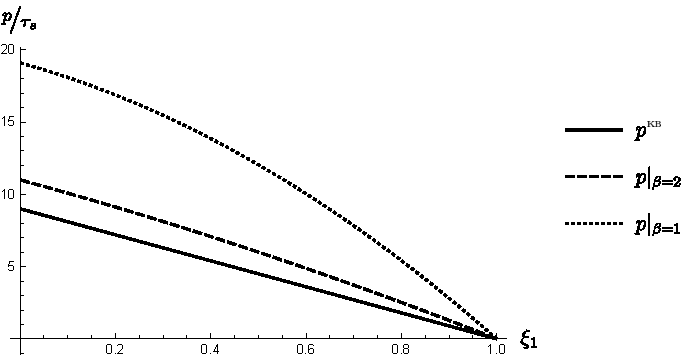
\includegraphics[scale=1.3]{./ch4/pressure}
    }
    \caption{Эпюры давления для случая плоского вязкопластического слоя}
    \label{fig:ch4/pressure}
\end{figure}анализе решения классической задачи Прандтля.

Используя то, что $\alpha(t) = V^2\left(t_*-t\right)^2 / \mathcal{S}_0$, где $\mathcal{S}_0$ -- площадь сечения слоя, можно установить зависимость между временем и стадией прессования:
\begin{equation}
  t_* - t \sim \frac{1}{\text{Eu}^{\nicefrac{1}{2\beta}}}\frac{\sqrt{\mathcal{S}_0}}{V}
\end{equation}
